\documentclass{article}

% set font encoding for PDFLaTeX or XeLaTeX
\usepackage{ifxetex}
\ifxetex
  \usepackage{fontspec}
\else
  \usepackage[T1]{fontenc}
  \usepackage[utf8]{inputenc}
  \usepackage{lmodern}
  \usepackage{graphicx}
  \usepackage{float}
\fi

% used in maketitle
\title{Cuestionario: Actividad 2}
\author{Luis Aarón Cerón Ramírez}
\usepackage[left=3cm,right=3cm,top=3cm,bottom=3cm]{geometry}

% Enable SageTeX to run SageMath code right inside this LaTeX file.
% documentation: http://mirrors.ctan.org/macros/latex/contrib/sagetex/sagetexpackage.pdf
% \usepackage{sagetex}

\begin{document}
\maketitle
\section{Preguntas sobre la actividad}
1.- Crear una gráfica que muestre la rapidez de los vientos y la rapidez de las ráfagas, como funciones del tiempo. ¿Cuáles son las horas del día con más viento?
\newline
Como se puede apreciar en la figura 1,la velocidad de las rafagas tienen mayor velocidad aproximadamente a las 36 horas, mientras que la mayor velocidad del viento se encuentra aproximadamente a las 78 horas y vuelven a tener un pico de la misma magnitud a las 95 horas.

\begin{figure}[H]
\centering
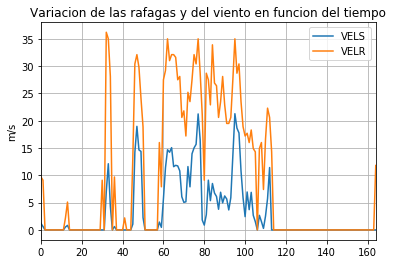
\includegraphics[scale=0.6]{rafagaviento.png}
\caption{Grafica de la velocidad de la rafaga y el viento en funcion del tiempo}
\label{figure: rafaga y viento}
\end{figure}

2.- Crear una gráfica con la dirección de los vientos como función del tiempo y comentar sobre los vientos dominantes en el sitio de estudio.

\begin{figure}[H]
\centering
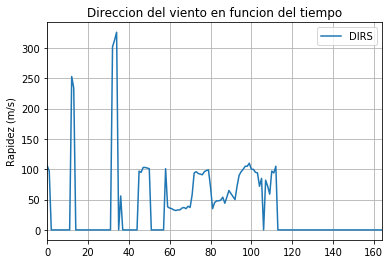
\includegraphics[scale=0.6]{direccion.png}
\caption{Grafica de la direccion del viento}
\label{figure: dirección viento}
\end{figure}

3.- Muestre el comportamiento de la Radiación Solar como función del tiempo. ¿Que puedes comentar?
\newline
Que la radiacion se comporta de manera poco intuitiva revisando la grafica, pues uno esperaria que los picos de radiacionse encontraran en las horas del dia por ejemplo a las doce horas y como se puede ver en la figura estos tienen sus picos aproximadamente de 20 a 30 horas los cuales son horas de la noche y la mañana.

\begin{figure}[H]
\centering
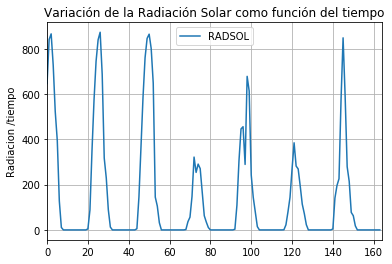
\includegraphics[scale=0.6]{radiacion.png}
\caption{Grafica de la radiacion}
\label{figure: Radiacion}
\end{figure}

4.- ¿Cuál es el lapso de temperatura diaria? (Diferencia entre la temperatura máxima y la mínima).
\newline
Las temperaturas maxima y minima fueron de $94.0^{\circ}$ y $8.6999999999999993^{\circ}$, por lo que el lapso de temperatura diaria es de $85.3^{\circ}$C.

5.- ¿Puedes comentar sobre la relación entre la temperatura y la humedad relativa?
\newline
Como se puede ver en la figura tanto la temperatura como la humedad relativa se mantienen constantes en el tiempo y con valores casi iguales en las dos, la diferencia mas notable es que ambas tienen picos al final delintervalo, siendo el de la temperatura el mas pronunciado.

\begin{figure}[H]
\centering
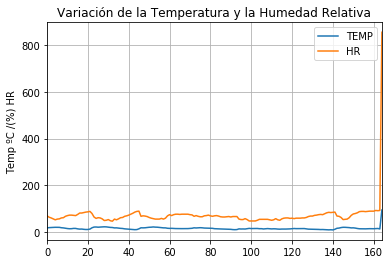
\includegraphics[scale=0.6]{relativa.png}
\caption{Grafica de la relación entre la temperatura y la humedad relativa}
\label{figure: temperatura y la humedad relativa}
\end{figure}

\section{Apendice}
1.- ¿Cuál es tu primera impresión de Jupyter Notebook?
\newline
Que se puede hacer mucho con pocas lineas de codigo
\newline
2.- ¿Se te dificultó leer código en Python?
\newline
Al nunca haber tenido un contacto con este tipo de lenguaje, se me dificulto bastante el poder trabajar con el realizando la actividad.
\newline
3.-  ¿En base a tu experiencia de programación en Fortran, que te parece el entorno de trabajar en Python?
\newline
Mas comodo para trabajar, por lo menos para realizar la actividad, aunque se necesita mucha mas practica.
\newline
4.- A diferencia de Fortran, ahora se producen las gráficas utilizando la biblioteca Matplotlib. ¿Cómo fue tu experiencia?.
\newline
Se me hizo mas facil realizar las graficas con python que con fortran.
\newline
5.- En general, ¿qué te pereció el entorno de trabajo en Python?
Bueno, bastante accesible, aunque al principio poco intuitivo.
\newline
6.- ¿Qué opinas de la actividad? ¿Estuvo compleja? ¿Mucho material nuevo? ¿Que le faltó o que le sobró? ¿Qué modificarías para mejorar?
\newline
En mi caso tuve bastante dificultades al principio, pero despues de buscar y preguntar me parecio mas sencilla, opino que el materialno fue demasiado, estubo bien como primer acercamiento.
\newline
7.- ¿Comentarios adicionales que desees compartir?
\newline
No tengo comentarios adicionales.











\end{document}
